%%% demothesis.tex ---
%%
%% Filename: demothesis.tex
%% Description:
%% Author: Ola Leifler
%% Maintainer:
%% Created: Thu Oct 14 12:52:20 2010 (CEST)
%% Version: $Id$
%% Version:
%% Last-Updated: Thu Apr 20 20:49:56 2017 (+0200)
%%           By: Ola Leifler
%%     Update #: 166
%% URL:
%% Keywords:
%% Compatibility:
%%
%%%%%%%%%%%%%%%%%%%%%%%%%%%%%%%%%%%%%%%%%%%%%%%%%%%%%%%%%%%%%%%%%%%%%%
%%
%%% Commentary:
%%
%%
%%
%%%%%%%%%%%%%%%%%%%%%%%%%%%%%%%%%%%%%%%%%%%%%%%%%%%%%%%%%%%%%%%%%%%%%%
%%
%%% Change log:
%%
%%
%% RCS $Log$
%%%%%%%%%%%%%%%%%%%%%%%%%%%%%%%%%%%%%%%%%%%%%%%%%%%%%%%%%%%%%%%%%%%%%%
%%
%%% Code:

\documentclass[msc,lith,english]{liuthesis}
%% Settings go in settings.tex
\include{settings}
\usepackage{rotating}
\usepackage{color}

% \usepackage{changebar}

\department{Institutionen för teknik och naturvetenskap}
\departmentenglish{Department of Science and Technology}
\departmentshort{ITN}

\externalsupervisor{Alexander Bock}
\supervisor{Emil Axelsson}
\examiner{Anders Ynnerman}
\titleenglish{Developing a Web GUI for rapid prototyping and public exhibitions}
\subtitleenglish{An OpenSpace project}
\titleswedish{En himla bra svensk titel}
\thesissubject{Datateknik}

\publicationyear{2017}
\currentyearthesisnumber{001}
% TODO: Fix publication date
\dateofpublication{2017-05-08}

\author{Klas Eskilson}

\begin{document}

\chapterstyle{VZ43}

\chapter{Introduction}
\label{cha:introduction}

% The introduction shall be divided into these sections:
Building an graphical user interface is a process that involves many steps. \source{Needs source about gui dev} \todo{what steps?} Being able to iterate several times is key, as this makes it possible to have user feedback tightly integrated into the process. Using a set of tools that allows for these iterations and simultaneously allows the developer to make quick changes is therefore a good step in the direction of building a well functioning user interface.

\section{Motivation}
\label{sec:motivation}

% This is where the studied problem is described from a general
% point of view and put in a context which makes it clear that
% it is interesting and well worth studying. The aim is to make
% the reader interested in the work and create an urge to
% continue reading.

Having a framework that allows for user interface components to be designed, developed and improved is a step into making OpenSpace \cite{jossos} a software application that may be used by a user with little or no previous experience.

This project is about using web technologies as the foundation of such a framework. Javascript, HTML and CSS \source{refer to standard} is used to built the user interface itself, and communication between the simulation and the user interface is done through web sockets \cite{fette2011websocket}. Evaluating this from a perspective of performance, usability and ease of development may tell if these technologies are well-suited in a C++ based application.

\section{Aim}
\label{sec:aim}

% What is the underlying purpose of the thesis project?

In this project, a C++ framework called Chromium Embedded Framework (CEF) is investigated and added to the OpenSpace application. The goal is to improve the pace at which the graphical user interface may be developed and improved. This, in turn, is to be able to improve the overall experience of using OpenSpace\todo{from what perspectives? improve how?}. The idea is to make OpenSpace more accessible and easier to understand.

Topics that will be investigated are communication, development pace, performance (in relationship to the other parts of the application and the GUI's impact on the performance in total) and extendibility.

% The aim of the project presented in this report is to

% \change{don't do this item list}
% \begin{itemize}
%   \item find technologies that are useful for graphical user interfaces,
%   \item implement a way of communication between the graphical user interface and the OpenSpace simulation,
%   \item implement a set of reusable components \unsure{is components clear enough?} that allows for an initial user interface to be implemented, and
%   \item implement a graphical user interface prototype.
% \end{itemize}

\section{Research questions}
\label{sec:research-questions}


% This is where the research questions are described.
% Formulate these as explicit questions, terminated with a
% question mark. A report will usually contain several different
% research questions that are somehow thematically connected.
% There are usually 2-4 questions in total.

In order to find an answer to the above mentionedw broad purpose and aim, the following questions will be answered.

\begin{enumerate}
  % Hur vill vi använda OpenSpace i framtiden?
  % Hur kan man med olika gui-approaches underlätta för slutanvändaren?
  \item What are the drawbacks and advantages of building a graphical user interface using web technologies? \label{q:drawbacks}
  \item How, if at all, can reusable components in a graphical user interface benefit development? \label{q:reuse}
  \item What are the drawbacks and advantages of communication internally and externally using web sockets? \label{q:websocket}
  \item How can different approaches to graphical user interface development change the end user's experience? \label{q:approach}
  \item How can graphical user interface development affect the future of a software product? \label{q:future}
\end{enumerate}


% Observe that a very specific research question almost always
% leads to a better thesis report than a general research question
% (it is simply much more difficult to make something good
% from a general research question.)

% The best way to achieve a really good and specific research
% question is to conduct a thorough literature review and get
% familiarized with related research and practice. This leads to
% ideas and terminology which allows one to express oneself
% with precision and also have something valuable to say in the
% discussion chapter. And once a detailed research question
% has been specified, it is much easier to establish a suitable
% method and thus carry out the actual thesis work much faster
% than when starting with a fairly general research question. In
% the end, it usually pays off to spend some extra time in the
% beginning working on the literature review. The thesis
% supervisor can be of assistance in deciding when the research
% question is sufficiently specific and well-grounded in related
% research.

\section{Delimitations}
\label{sec:delimitations}

% This is where the main delimitations are described. For
% example, this could be that one has focused the study on a
% specific application domain or target user group. In the
% normal case, the delimitations need not be justified.

In order to limit the scope of the project, user testing will not be conducted. The project will, in other words, \emph{not} be evaluated from a usability perspective.\unsure{should this be backed up by any arguments, or is this fine? guess it is fine.}

The components built and discussed here is assumed to be used on a regular, desktop or laptop computer. Neither hand held devices, touch interfaces nor immersive environments, such as a dome theatres or virtual reality devices, are part of the main target application.

\chapter{Theory}
\label{cha:theory}

% The main purpose of this chapter is to make it obvious for
% the reader that the report authors have made an effort to read
% up on related research and other information of relevance for
% the research questions. It is a question of trust. Can I as a
% reader rely on what the authors are saying? If it is obvious
% that the authors know the topic area well and clearly present
% their lessons learned, it raises the perceived quality of the
% entire report.

% After having read the theory chapter it shall be obvious for
% the reader that the research questions are both well
% formulated and relevant.

% The chapter must contain theory of use for the intended
% study, both in terms of technique and method. If a final thesis
% project is about the development of a new search engine for
% a certain application domain, the theory must bring up related
% work on search algorithms and related techniques, but also
% methods for evaluating search engines, including
% performance measures such as precision, accuracy and
% recall.

% The chapter shall be structured thematically, not per author.
% A good approach to making a review of scientific literature
% is to use \emph{Google Scholar} (which also has the useful function
% \emph{Cite}). By iterating between searching for articles and reading
% abstracts to find new terms to guide further searches, it is
% fairly straight forward to locate good and relevant
% information, such as \cite{test}.

% Having found a relevant article one can use the function for
% viewing other articles that have cited this particular article,
% and also go through the article’s own reference list. Among
% these articles on can often find other interesting articles and
% thus proceed further.

% It can also be a good idea to consider which sources seem
% most relevant for the problem area at hand. Are there any
% special conference or journal that often occurs one can search
% in more detail in lists of published articles from these venues
% in particular. One can also search for the web sites of
% important authors and investigate what they have published
% in general.

% This chapter is called either \emph{Theory, Related Work}, or
% \emph{Related Research}. Check with your supervisor.

\section{Web browsers and CEF}

Later in this paper, the implementation of a web browser within Openspace will be presented. But first, what a web browser is, the purpose of a web browser, a web browser's structure and some challenges that web browsers handles needs to be described.

For the sake of clarity, a web browser as discussed in this paper is a software application, or a part of one, that receives an arbitrary web resource in the form of an Uniform Resource Identifier (URI). \cite{jacobs2009uri} It then downloads this resource and presents it in an appropriate fashion.

\subsection{Structure}

I order to meet the requirements of a web browser and handling all the content that is should be supported according to the HTML 5 standard \cite{html}, a web browser becomes an application with a complicated structure. Among several things, media download, web rendering and user interaction should all happen in the same application. All this preferably with little to no delay and without disrupting any of the other tasks.

In the CEF and Chromium projects, the sollution is handling most tasks through a mutli-processes, multi threaded approach. This allows multiple tasks to be handled simultaneously. \cite{cefusage} A user's interactions should ideally not disrupt the playback of a video or a sound, for instance.

\subsection{Executables in CEF}

\begin{figure}[h]\label{fig:processes}
\centering
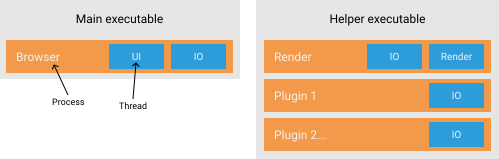
\includegraphics[width=0.9\linewidth]{./figures/process.pdf}
\caption{\emph{An overview of the two-executable structure with processes and threads.}}
\end{figure}

CEF has support for two different executable models. The implementation uses either one or two separate executables for its sub processes. An overview can be seen in figure \ref{fig:processes}. The processes are launched with different command line arguments that determine the purpose of the launched process. These arguments get sent to either the \texttt{CefExecuteProcess}, which then takes care of determining what needs to be done. The single-executable structure is supported on Windows and Linux system, but not on Macos systems. \cite{cefusage}

In a single-executable implementation of CEF, the return code of \texttt{CefExecuteProcess} is used to determine wether or not execution of that process should be terminated. In a two-executable implementation, the main executable (that also runs the rest of the application) initializes CEF with an option parameter declaring the location of the sub-process executable. In this case, the sub-executable is a single-purpose executable that does little else than calling \texttt{CefExecuteProcess} to allow CEF to handle the incoming task. By using dynamic, shared libraries, the double-executable approach does not necessarily increase the application size, as the two executables share the CEF library.

A potential drawback of a single-executable implementation is that the implementation becomes sensitive to where \texttt{CefExecuteProcess} gets called. If it is late in the application bootup, this may cause delays in CEF's sub-process spawning.

\subsection{Processes in CEF}

In CEF, each different thread and process have separate purposes. They handle different tasks. Although the there might be similarities between the tasks, they are distinct. The main, "browser", process handles window management (towards the host operating system), painting and network access. This process is the same as the host application, where the rest of the application's logic is run.

Another process is called the render process. This is where Blink rendering and javascript execution happens. Blink is Chromium's web rendering engine - it takes formatting information such as CSS style sheets and transform it into the visual result that eventually will be shown. \cite{blink} For safety and robustness, each unique combination of URL scheme and origin will trigger a new render process to be spawned. A URL scheme is the initial part of the URL, usually describing which protocol that should be used. It may look like \texttt{https}, \texttt{http} or \texttt{ftp}. The origin is in this case the domain name or IP address of the URL. By default, Chromium does not separate web pages from different sub domains (\texttt{one.example.com} and \texttt{two.example.com}) or ports (\texttt{example.com:80} and \texttt{example.com:443}). \cite{processes} This separation and reusability of processes is considered to give a good balance of safety and computing resource usage at the same time as allowing instances of different web pages from the same web site to access each other according to the enforced security policy. \cite{network10same}

The other processes that may be spawned by CEF are related to so called plugins. These might be if a web site wants to show content that are developed by a third party, for instance. This might be Flash content, Java aplets, or similar. GPU powered content are also being handled by a separate process.

An overview of the different processes together with its executables and threads can be seen in figure \ref{fig:processes}.

\subsection{Threads in CEF}

Each process in CEF is also multi threaded. This is where the multi-dimensional parallelism structure of CEF comes in. The different threads handle different aspects of constructing the requested web page. As mentioned in \cite{cefusage}, there are many different threads used by different processes. The most common ones are:

\begin{itemize}
  \item The \textbf{UI} thread. This is the main thread of the browser process. It is the thread where the function \texttt{CefInitialize} is called to initialize the CEF framework.
  \item The \textbf{IO} thread, where inter-process messaging is handled and where network messages are processed.
  \item The \textbf{renderer} thread, which is the main thread of the renderer process.
\end{itemize}

\subsection{Challenges}

\section{Web sockets}

The Web socket technology is an extension of TCP sockets made for two-way communication between a client and a host. The protocol uses TCP \cite{postel1981transmission} as the transport layer. By using HTTP to complete a handshaking process, a persistent connection between the peers may be esatablished. This means that no further handshaking is required, since the TCP connection remains open. Web sockets are essentially a layer on top of TCP that adds web targeted security model, an addressing and naming mechanism to support several services on one port, a framing mechanism to describe the messages and some other more handshaking related mechanisms. \cite{fette2011websocket}

Arbitrary UTF-8 \cite{RFC3629} text messages or binary data may be sent over the connection. These are interpeted as standalone messages, and the peers should treat them as such. This differs from raw sockets where the messaging back and forth can be seen as streams, and where some sort of breaking character or sequence must be used to distinguish messages from each other. The web socket frame header contains details of how long the message is, and this tells the clients how to interpret the received frames and where the frames end.

Web socket supports both unecrypted messages with the uri scheme \texttt{ws://} and encrypted messages over TLS \cite{RFC5246} with the control sequence \texttt{wss://}.

\subsection{Establishing and closing connections}

In order to establish a web socket connection, a handshake process using HTTP is used. The client requests a protocol upgrade to the web socket protocol. The successfull response to the client-initiated request is a HTTP 101 response, stating that the used protocol should be switched. \cite[section 10.1.2]{RFC2616} See \cite{RFC2616} for further details on the client's request.

The server also has mechanisms to proove the validity of the response. This is done by combining two pieces of information; the \texttt{Sec-WebSocket-Key} value from the client's request and the fixed string \texttt{258EAFA5-E914-47DA-95CA-C5AB0DC85B11}. By concatenating these two and base64-encoding \cite{base64} the hash of the combination generated using SHA-1 \cite{RFC3174}, the client may verify the server's response. The fixed string is assumed to not be used by any other protocol. This should validate the connection, so that the client knows that the server is compatible.

To close a connection, another handshaking mechanism is in place. This is on top of the TCP connection closing mechanism, as that is not always end-to-end reliable and connections may be in a half-closed state with messages not yet fully transmitted. \cite[section 4.2.2.13]{RFC1122} The web socket closing mechanism relies on a confirmation, where the first peer initiates the closing by sending a close frame and the second peer sends a close frame in response. This way, the number of cases where data is lost in a half-closed state is reduced. Both peers may initiate the close handshake simultaneously.

When closing the connection, an optional reason code may be provided to explain why the connection is being closed. This can be used to allow the other peer to make a good decision in how to act after the closing.

\section{Javascript UI framework React}

React is an open source javascript framework for building user interfaces. It manipulates the web browser's document object model (DOM) to provide the developer with an API (application programming interface) to build the interface. It uses a declarative paradigm to allow the developer to create components. \cite{react} These components may be reused and are highly configurable for the developer.

In React, the user interface can be described as a function of the the application's state. In a mathematical context, this may be described as $UI = f(state)$. The state of a React component is either owned by itself, in which case it is called \emph{state}, or it may be passed down from the parent component, in which case it is called \emph{props}, or it may be a combination of the two.

React components may be written is different ways. Either using the ES5-style \cite{es5} \texttt{React.createReactClass}, using ES6-style \cite{es6} class extending or as so-called pure functional components, which essentially are functions returning valid React elements.

\subsection{JSX}\label{sec:jsx}

How React elements are written may vary, too. With React, a XML-like javascript subset called JSX was developed. See Listing~\ref{lst:jsx} for a simple example. The second option is using the React API with the \texttt{React.createElement} method, see Listing~\ref{lst:element}.

\begin{lstlisting}[caption={Simple JSX example snippet},label=lst:jsx]
const element = <h1>Hello, world!</h1>;
\end{lstlisting}

\begin{lstlisting}[caption={Usage of React.createElement},label=lst:element]
// React.createElement(component, props, children);
React.createElement('div', null, 'Hello World');
\end{lstlisting}

By removing the need for advanced API usage, such as \texttt{React.createElement}, and replacing it with the XML-like syntax, JSX allows the developer to understand what the end component will look like faster. JSX also comes with other features. One is HTML injection prevention to ensure no malicious HTML gets injected to the page. Another is a simplified syntax for dynamic element attributes, see Listing~\ref{lst:attributes}.

\begin{lstlisting}[caption={Element attributes in JSX},label=lst:attributes]
const url = 'image.png';
const element = <img src={url} />;
\end{lstlisting}

\section{Transpiling}

In order to use modern javascript features without loosing support for older web browsers and servers that doesn't yet support these features, a technique called \emph{transpiling} (combination of \emph{transformation} and \emph{compilation}) can be used. \cite[p. 3-4]{youdontknowjs} These features are amongst others classes and inheritance, modules, arrow functions and object destructuring. The technique is also used for JSX (see section \ref{sec:jsx} JSX).

This technique transforms the newer syntax to an older, more well-supported syntax automatically. This is oftenly done through adding a build-step into the development workflow, similar to linting and other operations. This process isn't needed for all new javascript features, as some can be added to the programming environment by the developer through another technique called polyfills. \cite[p. 4-5]{youdontknowjs}

\section{Data serialization: JSON}

JSON (JavaScript Object Notation) is a data format useful for serializing arbitrary data types into a transport-friendly format. It is a text format, meaning it is readable. In it, strings, numbers, booleans, and null-values can be stored. Structural types are arrays of objects. The syntax is derived from the object and array syntax of javascript. \cite{json}

\todo[inline]{what else?}

%%% lorem.tex ---
%%
%% Filename: lorem.tex
%% Description:
%% Author: Ola Leifler
%% Maintainer:
%% Created: Wed Nov 10 09:59:23 2010 (CET)
%% Version: $Id$
%% Version:
%% Last-Updated: Wed Nov 10 09:59:47 2010 (CET)
%%           By: Ola Leifler
%%     Update #: 2
%% URL:
%% Keywords:
%% Compatibility:
%%
%%%%%%%%%%%%%%%%%%%%%%%%%%%%%%%%%%%%%%%%%%%%%%%%%%%%%%%%%%%%%%%%%%%%%%
%%
%%% Commentary:
%%
%%
%%
%%%%%%%%%%%%%%%%%%%%%%%%%%%%%%%%%%%%%%%%%%%%%%%%%%%%%%%%%%%%%%%%%%%%%%
%%
%%% Change log:
%%
%%
%% RCS $Log$
%%%%%%%%%%%%%%%%%%%%%%%%%%%%%%%%%%%%%%%%%%%%%%%%%%%%%%%%%%%%%%%%%%%%%%
%%
%%% Code:

\chapter{Method}
\label{cha:method}

% In this chapter, the method is described in a way which shows how the
% work was actually carried out. The description must be precise and
% well thought through. Consider the scientific term
% replicability. Replicability means that someone reading a scientific
% report should be able to follow the method description and then carry
% out the same study and check whether the results obtained are
% similar. Achieving replicability is not always relevant, but precision
% and clarity is.

% Sometimes the work is separated into different parts, e.g.  pre-study,
% implementation and evaluation. In such cases it is recommended that
% the method chapter is structured accordingly with suitable named
% sub-headings.

The project can be divided into three major parts; the web browser, the server and simulation control, and the GUI. They were roughly developed in this order, with some overlapping and fixes.

\section{Web browser}

Initially in the project, the requirements and structure of CEF was investigated. This was to as quick as possible determine wether or not including CEF in Openspace and its OpenGL structure would work. It was found that both Openspace and CEF uses Cmake as the build system-of-choice. This allowed the work to continue.

CEF provided Cmake bootstraping helpers, to download the binary library files for the framework. Depending on what platform and architecture that the developer was using, the helper automatically detected this and downloaded the needed binaries from CEF's web page. By combining this with Openspace's Cmake module system, a web browser module was added to the build process. This downloaded, unpacked and included the needed CEF files. Some compiler flags that CEF's Cmake instructions inserted into the build process were not supported by Openspace and created issues at build time. Manually removing these from the downloaded CEF structure resolved that issue.

When the project was successfully compiling with the CEF includes, the next step was to start implementing the rendering mechanism for the the web browser. This was done by using a rendering method called Off Screen Rendering (OSR) in CEF, that allows the developer to use a callback for whenever the web page needs to be rerendered. After the rendering was in place, the user interaction was the next step. This was done by using the event handlers that already exists in Openspace and sending them to CEF. The key events, however, needed to be handled differently. The modifier keys, such as control, shift and alt, needed to be translated from \todo{what?} to \todo{what?} in order to CEF to understand them.

When rendering and user interaction was in place, the next step was to implement a web socket interface.

Most of the documentation of CEF is focused on building a new application, not so much to implement it into an existing code base. \todo{move this to discussion or so}

\section{Socket server and simulation control}

In order to allow the GUI to control the simulation in Openspace, a way of communicating between the user's interactions in the GUI and the simulation engine needed to be put into place. CEF and Chromium has a fully working web socket client built in, which is why web socket was considered a good option for communication.

Two different web socket libraries were considered: \emph{Libwebsockets} and \emph{Websocket++}. Libwebsockets is, however, single threaded and written in C, not C++ like Openspace. \cite{lwssingle} Websocket++ is written in C++ and has built-in multithreaded support. By using the already existing TCP socket abstraction that existed in Openspace, websocket support was added.

\todo[inline]{write about server}

\section{GUI development}

\todo[inline]{write about gui}

%%%%%%%%%%%%%%%%%%%%%%%%%%%%%%%%%%%%%%%%%%%%%%%%%%%%%%%%%%%%%%%%%%%%%%
%%% lorem.tex ends here

%%% Local Variables:
%%% mode: latex
%%% TeX-master: "demothesis"
%%% End:

\chapter{Results}
\label{cha:results}

% This chapter presents the results. Note that the results are presented
% factually, striving for objectivity as far as possible.  The results
% shall not be analyzed, discussed or evaluated.  This is left for the
% discussion chapter.

% In case the method chapter has been divided into subheadings such as
% pre-study, implementation and evaluation, the result chapter should
% have the same sub-headings. This gives a clear structure and makes the
% chapter easier to write.

% In case results are presented from a process (e.g. an implementation
% process), the main decisions made during the process must be clearly
% presented and justified. Normally, alternative attempts, etc, have
% already been described in the theory chapter, making it possible to
% refer to it as part of the justification.

\section{Web browser}

The resulting web browser is implemented in two ways. The first as a so called screen space browser. This is a browser window within the Openspace window that can be moved around and placed on the screen where the user wants it. See figure \ref{fig:screenspace}.

\begin{figure}[!h]
\centering
\includegraphics[width=0.7\linewidth]{./figures/screenspace.png}
\caption{\emph{The screen space browser with controls. The browser window is showing a video from the Openspace Youtube page.}}\label{fig:screenspace}
\end{figure}

The second is the screen-covering GUI browser. This is a transparent browser layer that covers the entire Openspace window. This is used to render the GUI on screen. See figure \ref{fig:guiprocess} for an early screen shot in the process of creating the GUI. While the screen space browser has a dynamic window size, allowing it to be changed as the user wants, the GUI browser's dimensions change as the window is resized.

\begin{figure}[!h]
\centering
\includegraphics[width=0.7\linewidth]{./figures/guiprocess.png}
\caption{\emph{A screen shot from the GUI development, showing a misaligned sidebar and stringified JSON response from the simulation.}}\label{fig:guiprocess}
\end{figure}

\subsection{Event handling and interaction}\label{sec:interaction}

To handle events and interactions from the user, an event handler was created. This is a C++ class that holds a reference to a single active browser window within Openspace. This can be either a screen space window or the GUI window. This event handler listens to the events that gets captured by Openspace, which include keyboard button clicks, mouse movement, mouse button clicks and mouse scroll wheel movement. These get sent to the active browser windows using corresponding public methods.

To determine whether or not a mouse event should be captured, and blocked from triggering other parts of Openspace, a transparency layer mask is stored by each browser window. This is based on the assumption that an interaction over a transparent area won't trigger anything on the web page. See figure \ref{fig:maskweb} for an example view in the GUI and figure \ref{fig:maskmask} for its corresponding layer mask.

\begin{figure}[!h]
  \centering
  \subfloat[The GUI as it looks in Openspace, overlooking the surface of Mars.]{\includegraphics[width=0.45\textwidth]{./figures/maskweb.png}\label{fig:maskweb}}
  \hfill
  \subfloat[The layer mask. The black area will capture mouse clicks and mouse wheel movement.]{\fbox{\includegraphics[width=0.45\textwidth]{./figures/maskmask.png}\label{fig:maskmask}}}
  \caption{The layer interaction mask}
\end{figure}

The layer mask is stored as a one-dimensional C++ array, and is updated every time the GUI is re-rendered. See more about the rendering in section \ref{sec:rendering}. When a user clicks inside the area marked as non-transparent, this will be sent to the GUI, and the event is captured. If the user clicks outside the area, the event will be ignored by the GUI, and the event trickles on within Openspace.

To get the index $i$ in the one-dimensional layer mask array from the coordinates $x$ and $y$, equation \ref{eq:coordtoidx} is used. Here, $W$ is the width of the browser window. This equation is used to decide whether or not the user's interaction is within an active area of the browser or not, as the position is given as coordinates in Openspace's event handlers.

\begin{equation}\label{eq:coordtoidx}
  i = x + y \cdot W
\end{equation}

\todo{figure with hit and miss on mask? is it needed?}

Keyboard button events, typing, is always sent to the GUI and never blocked. The phenomena caused by this, such as keyboard shortcuts getting unintentionally triggered, will later be discussed. \todo{discuss double effects of some key presses}

\begin{figure}[!h]
\centering
\includegraphics[width=0.9\linewidth]{./figures/maskupdate.png}
\caption{\emph{Overview of the mask update and user interaction process.}}\label{fig:maskupdate}
\end{figure}

When a browser window gets repainted, a buffer stored in the web renderer gets updated, see \ref{sec:rendering}. At this time, the layer mask also gets updated. To do this, the alpha channel of the RGBA values are extracted. If the alpha value of a pixel is non-zero, meaning that it is untransparent, this is considered a pixel that will capture the mouse events. See the life cycle of the interaction decision process in figure \ref{fig:maskupdate}.

\subsection{Rendering}\label{sec:rendering}

\begin{figure}[!h]
\centering
\includegraphics[width=0.9\linewidth]{./figures/rendering.png}
\caption{\emph{Overview of the rendering process.}}\label{fig:rendering}
\end{figure}

The rendering is a two-part process. First, CEF renders the web page to a buffer. This buffer is then copied on the working memory from CEF to the web browser implementation in Openspace. The buffer is then copied, each frame, to the GPU in the OpenGL pipeline in order to be drawn on the screen. The copying from CEF to Openspace is triggered only when the web page needs to be rendered, and the stored buffer is used until it gets updated and replaced by a new copy. See figure \ref{fig:rendering} for an overview of the steps in the rendering process.

To reduce the computing power needed, CEF only updates the buffer when something on the web page gets changed and a repaint of the web page is needed. This can be a colour changing, text changing, box moving or anything similar. Regardless of the magnitude of the change or the cause of this change, the whole buffer gets replaced. This affects both the transparency mask mentioned in section \ref{sec:interaction} and the buffer that gets copied to the GPU for rendering. Depending on the internal bandwidth of the computer, this copying from the RAM to the GPU might be a time consuming task, affecting the performance of the simulation. The implications of this will be discussed later. \todo{discuss ram to gpu copying}

\section{Socket server and simulation control}
\section{GUI development}

\include{discussion}
\include{conclusion}
\printbibliography

\end{document}

%%%%%%%%%%%%%%%%%%%%%%%%%%%%%%%%%%%%%%%%%%%%%%%%%%%%%%%%%%%%%%%%%%%%%%
%%% demothesis.tex ends here

